\documentclass[nooutcomes]{ximera}
\graphicspath{{./}{thePythagoreanTheorem/}{deMoivreSavesTheDay/}{complexNumbersFromDifferentAngles/}{trianglesOnACone/}{cityGeometry/}{EuclidAndGeometry/}}

\usepackage{gensymb}
\usepackage[margin=1in]{geometry}

%\usepackage{hyperref}


\usepackage{tikz}
\usepackage{tkz-euclide}
\usetkzobj{all}
\tikzstyle geometryDiagrams=[ultra thick,color=blue!50!black]
\newcommand{\tri}{\triangle}
\renewcommand{\l}{\ell}
\renewcommand{\P}{\mathcal{P}}
\newcommand{\R}{\mathbb{R}}
\newcommand{\Q}{\mathbb{Q}}

\newcommand{\Z}{\mathbb Z}
\newcommand{\N}{\mathbb N}
\newcommand{\ph}{\varphi}

\renewcommand{\vec}{\mathbf}
\renewcommand{\d}{\,d}


%\counterwithin*{question}{section} <- This didn't work



%% Egyptian symbols

\usepackage{multido}
\newcommand{\egmil}[1]{\multido{\i=1+1}{#1}{\includegraphics[scale=.1]{egyptian/egypt_person.pdf}\hspace{0.5mm}}}
\newcommand{\eghuntho}[1]{\multido{\i=1+1}{#1}{\includegraphics[scale=.1]{egyptian/egypt_fish.pdf}\hspace{0.5mm}}}
\newcommand{\egtentho}[1]{\multido{\i=1+1}{#1}{\includegraphics[scale=.1]{egyptian/egypt_finger.pdf}\hspace{0.5mm}}}
\newcommand{\egtho}[1]{\multido{\i=1+1}{#1}{\includegraphics[scale=.1]{egyptian/egypt_lotus.pdf}\hspace{0.5mm}}}
\newcommand{\eghun}[1]{\multido{\i=1+1}{#1}{\includegraphics[scale=.1]{egyptian/egypt_scroll.pdf}\hspace{0.5mm}}}
\newcommand{\egten}[1]{\multido{\i=1+1}{#1}{\includegraphics[scale=.1]{egyptian/egypt_heel.pdf}\hspace{0.5mm}}}
\newcommand{\egone}[1]{\multido{\i=1+1}{#1}{\includegraphics[scale=.1]{egyptian/egypt_stroke.pdf}\hspace{0.5mm}}}
\newcommand{\egyptify}[7]{
 \multido{\i=1+1}{#1}{\includegraphics[scale=.1]{egyptian/egypt_person.pdf}\hspace{0.5mm}}
 \multido{\i=1+1}{#2}{\includegraphics[scale=.1]{egyptian/egypt_fish.pdf}\hspace{0.5mm}}
 \multido{\i=1+1}{#3}{\includegraphics[scale=.1]{egyptian/egypt_finger.pdf}\hspace{0.5mm}}
 \multido{\i=1+1}{#4}{\includegraphics[scale=.1]{egyptian/egypt_lotus.pdf}\hspace{0.5mm}}
 \multido{\i=1+1}{#5}{\includegraphics[scale=.1]{egyptian/egypt_scroll.pdf}\hspace{0.5mm}}
 \multido{\i=1+1}{#6}{\includegraphics[scale=.1]{egyptian/egypt_heel.pdf}\hspace{0.5mm}}
 \multido{\i=1+1}{#7}{\includegraphics[scale=.1]{egyptian/egypt_stroke.pdf}\hspace{0.5mm}}
 \hspace{.5mm}
}





\title{Measuring}

\begin{document}
\begin{abstract}
    We begin to explore Ancient Greek thinking about geometry.
\end{abstract}
\maketitle

\begin{definition}
Let's say one segment $AB$ {\bf measures} another segment $CD$ is we can find a whole number $N$ so that $CD$ is composed of exactly $N$ copies of $AB$.
\end{definition}

\begin{problem}
Draw $AB$ of length $3$ cm and $CD$ of length $12$cm, and show in your drawing that $AB$ measures $CD$.
\end{problem}

\begin{definition}
Let's say that two segments $AB$ and $CD$ are {\bf commensurable} if we can find another segment $EF$ so that $EF$ measures both $AB$ and $CD$. Otherwise, we will say that $AB$ and $CD$ are {\bf incommensurable}
\end{definition}


\begin{problem}
Find a pair of line segments which are commensurable. Explain why the Pythagoreans could have concluded that every pair of line segments must be commensurable.
\end{problem}

\begin{problem}
Find a pair of line segments which are incommensurable. Explain why the Pythagoreans were distressed by such a discovery.
\end{problem}

\begin{definition}[From Euclid's Elements]
A straight line (segment) is said to have been cut in extreme and mean ratio when, as the whole line is to the greater segment, so is the greater to the less.
\end{definition}

\begin{problem}
What is this definition saying? Express the ratio using modern mathematical symbols.
\begin{center}
\begin{tikzpicture}
\draw (0,0)--(5,0);
\draw[fill=black] (0,0) circle (2pt);
\node at (0,0.5) {$A$};
\draw[fill=black] (3.0902,0) circle (2pt);
\node at (3.0902,0.5) {$C$};
\draw[fill=black] (5,0) circle (2pt);
\node at (5,0.5) {$B$};
\end{tikzpicture}
\end{center}
\end{problem}

\begin{question}
Can you find any examples of extreme and mean ratio in the diagram of a regular pentagon? Prove your claim!
\begin{center}
\begin{tikzpicture}
	\node[regular polygon, 
	draw,
	minimum size=4cm] (p) at (0,0) {};
	\foreach \x in {1,2,...,5}
  		\fill (p.corner \x) circle[radius=2pt];
	\node[above] (g) at (p.north) {$G$};
	\node[above right] at (p.18) {$F$};
	\node[right] (e) at (p.306) {$E$};
	\node[left] at (p.234) {$D$};
	\node[above left] at (p.162) {$H$};
	\path[draw, name path=L1] (p.90)--(p.306);
	\path[draw, name path=L2] (p.18)--(p.234);
	\draw[name intersections = {of = L1 and L2, by = x}][fill] (x) circle (2pt) node[above left, outer sep=0pt] {$A$};
\end{tikzpicture}
\end{center}
%\begin{center} 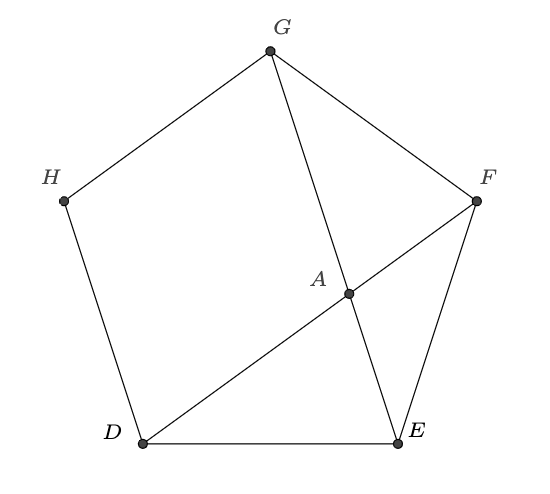
\includegraphics[scale=0.8]{./PythagorasAndEarlyGreek/pentagon.png} \end{center}
\end{question}

\end{document}